\newcommand{\ww}{0.32333} 
\begin{figure}[H] 
    \captionsetup[subfloat]{justification=raggedright,singlelinecheck=false, position=bottom,labelformat=empty} % 
    \subfloat[Wielkość obrazu O1: 500x512]{
       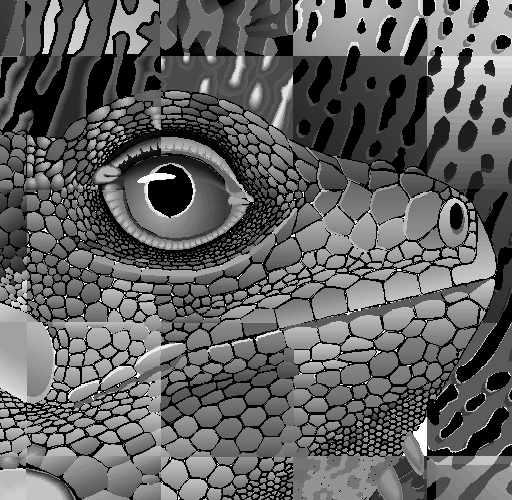
\includegraphics[width=\ww\linewidth]{../zad1/img3/O1___.png}}  \hfill% 
    \subfloat[Wielkość obrazu: 500x512\\ Wielkość maski: 3x 3x]{
       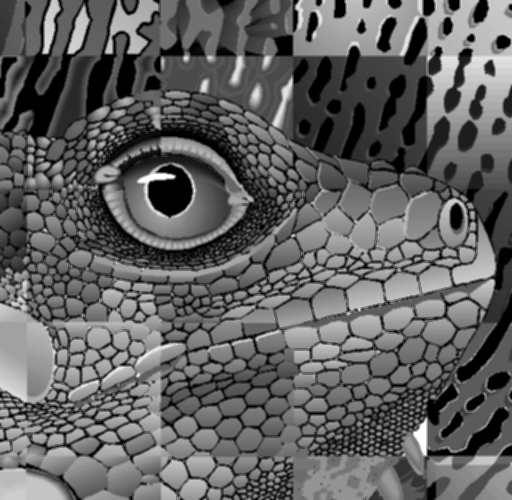
\includegraphics[width=\ww\linewidth]{../zad1/img3/O1_Md.png}}  \hfill% 
    \subfloat[Wielkość obrazu: 500x512\\ Wielkość maski: 3x 3x]{
       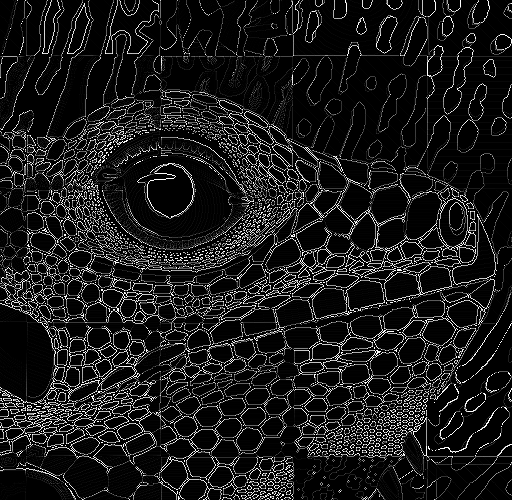
\includegraphics[width=\ww\linewidth]{../zad1/img3/O1_Mg.png}}  \\ 
    \subfloat[Wielkość obrazu O1: 500x512]{
       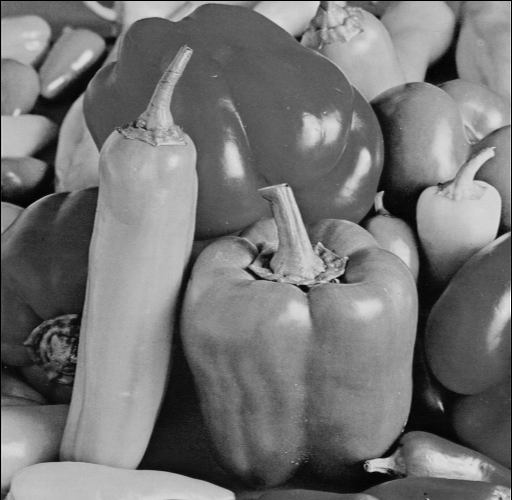
\includegraphics[width=\ww\linewidth]{../zad1/img6/O1___.png}}  \hfill% 
    \subfloat[Wielkość obrazu: 500x512\\ Wielkość maski: 3x 3x]{
       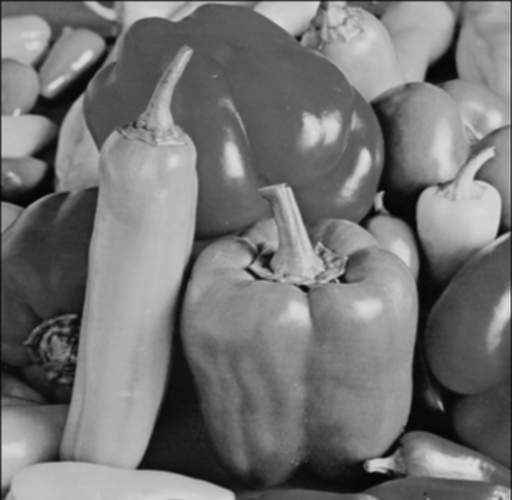
\includegraphics[width=\ww\linewidth]{../zad1/img6/O1_Md.png}}  \hfill% 
    \subfloat[Wielkość obrazu: 500x512\\ Wielkość maski: 3x 3x]{
       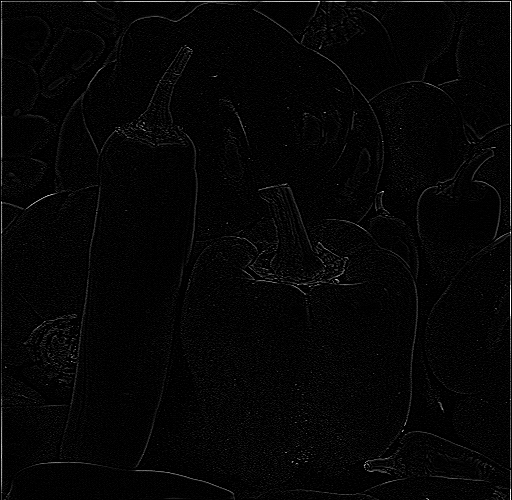
\includegraphics[width=\ww\linewidth]{../zad1/img6/O1_Mg.png}}
\caption{Porownanie}  
\label{fig:../zad1/result_3_6.tex} 
\end{figure} 
\let\ww\undefined 
maski użyte do filtracji obrazu:
$$
\begin{array}{cc}
Md =  \begin{bmatrix}  \frac{1}{9} & \frac{1}{9} & \frac{1}{9}\\[6pt]
 \frac{1}{9} & \frac{1}{9} & \frac{1}{9}\\[6pt]
 \frac{1}{9} & \frac{1}{9} & \frac{1}{9} \end{bmatrix} 
&
Mg =  \begin{bmatrix}  0 & -1 & 0\\[6pt]
 -1 & 4 & -1\\[6pt]
 0 & -1 & 0 \end{bmatrix} 
\end{array}
$$